\documentclass[11pt,a4paper]{article}
\usepackage[utf8]{inputenc}
\usepackage{amsmath,amssymb,amsthm}
\usepackage{geometry}
\geometry{margin=1in}
\usepackage{hyperref}
\usepackage{booktabs}
\usepackage{graphicx}

\title{Universitas Pandrosion: Paper~101ABC \\
Synthesis of the Algorithmic Closure \\
\large From $O(d^{2}\log^{2}d)$ to $O(d \log d)$ Las~Vegas on Kostlan--Smale}
\author{I. Besevic}
\date{April 2026}

\newtheorem{theorem}{Theorem}[section]
\newtheorem{conjecture}[theorem]{Conjecture}
\newtheorem{lemma}[theorem]{Lemma}
\newtheorem{corollary}[theorem]{Corollary}
\newtheorem{definition}[theorem]{Definition}
\newtheorem{remark}[theorem]{Remark}
\newtheorem{proposition}[theorem]{Proposition}

\begin{document}
\maketitle

\begin{figure}[h!]
\centering
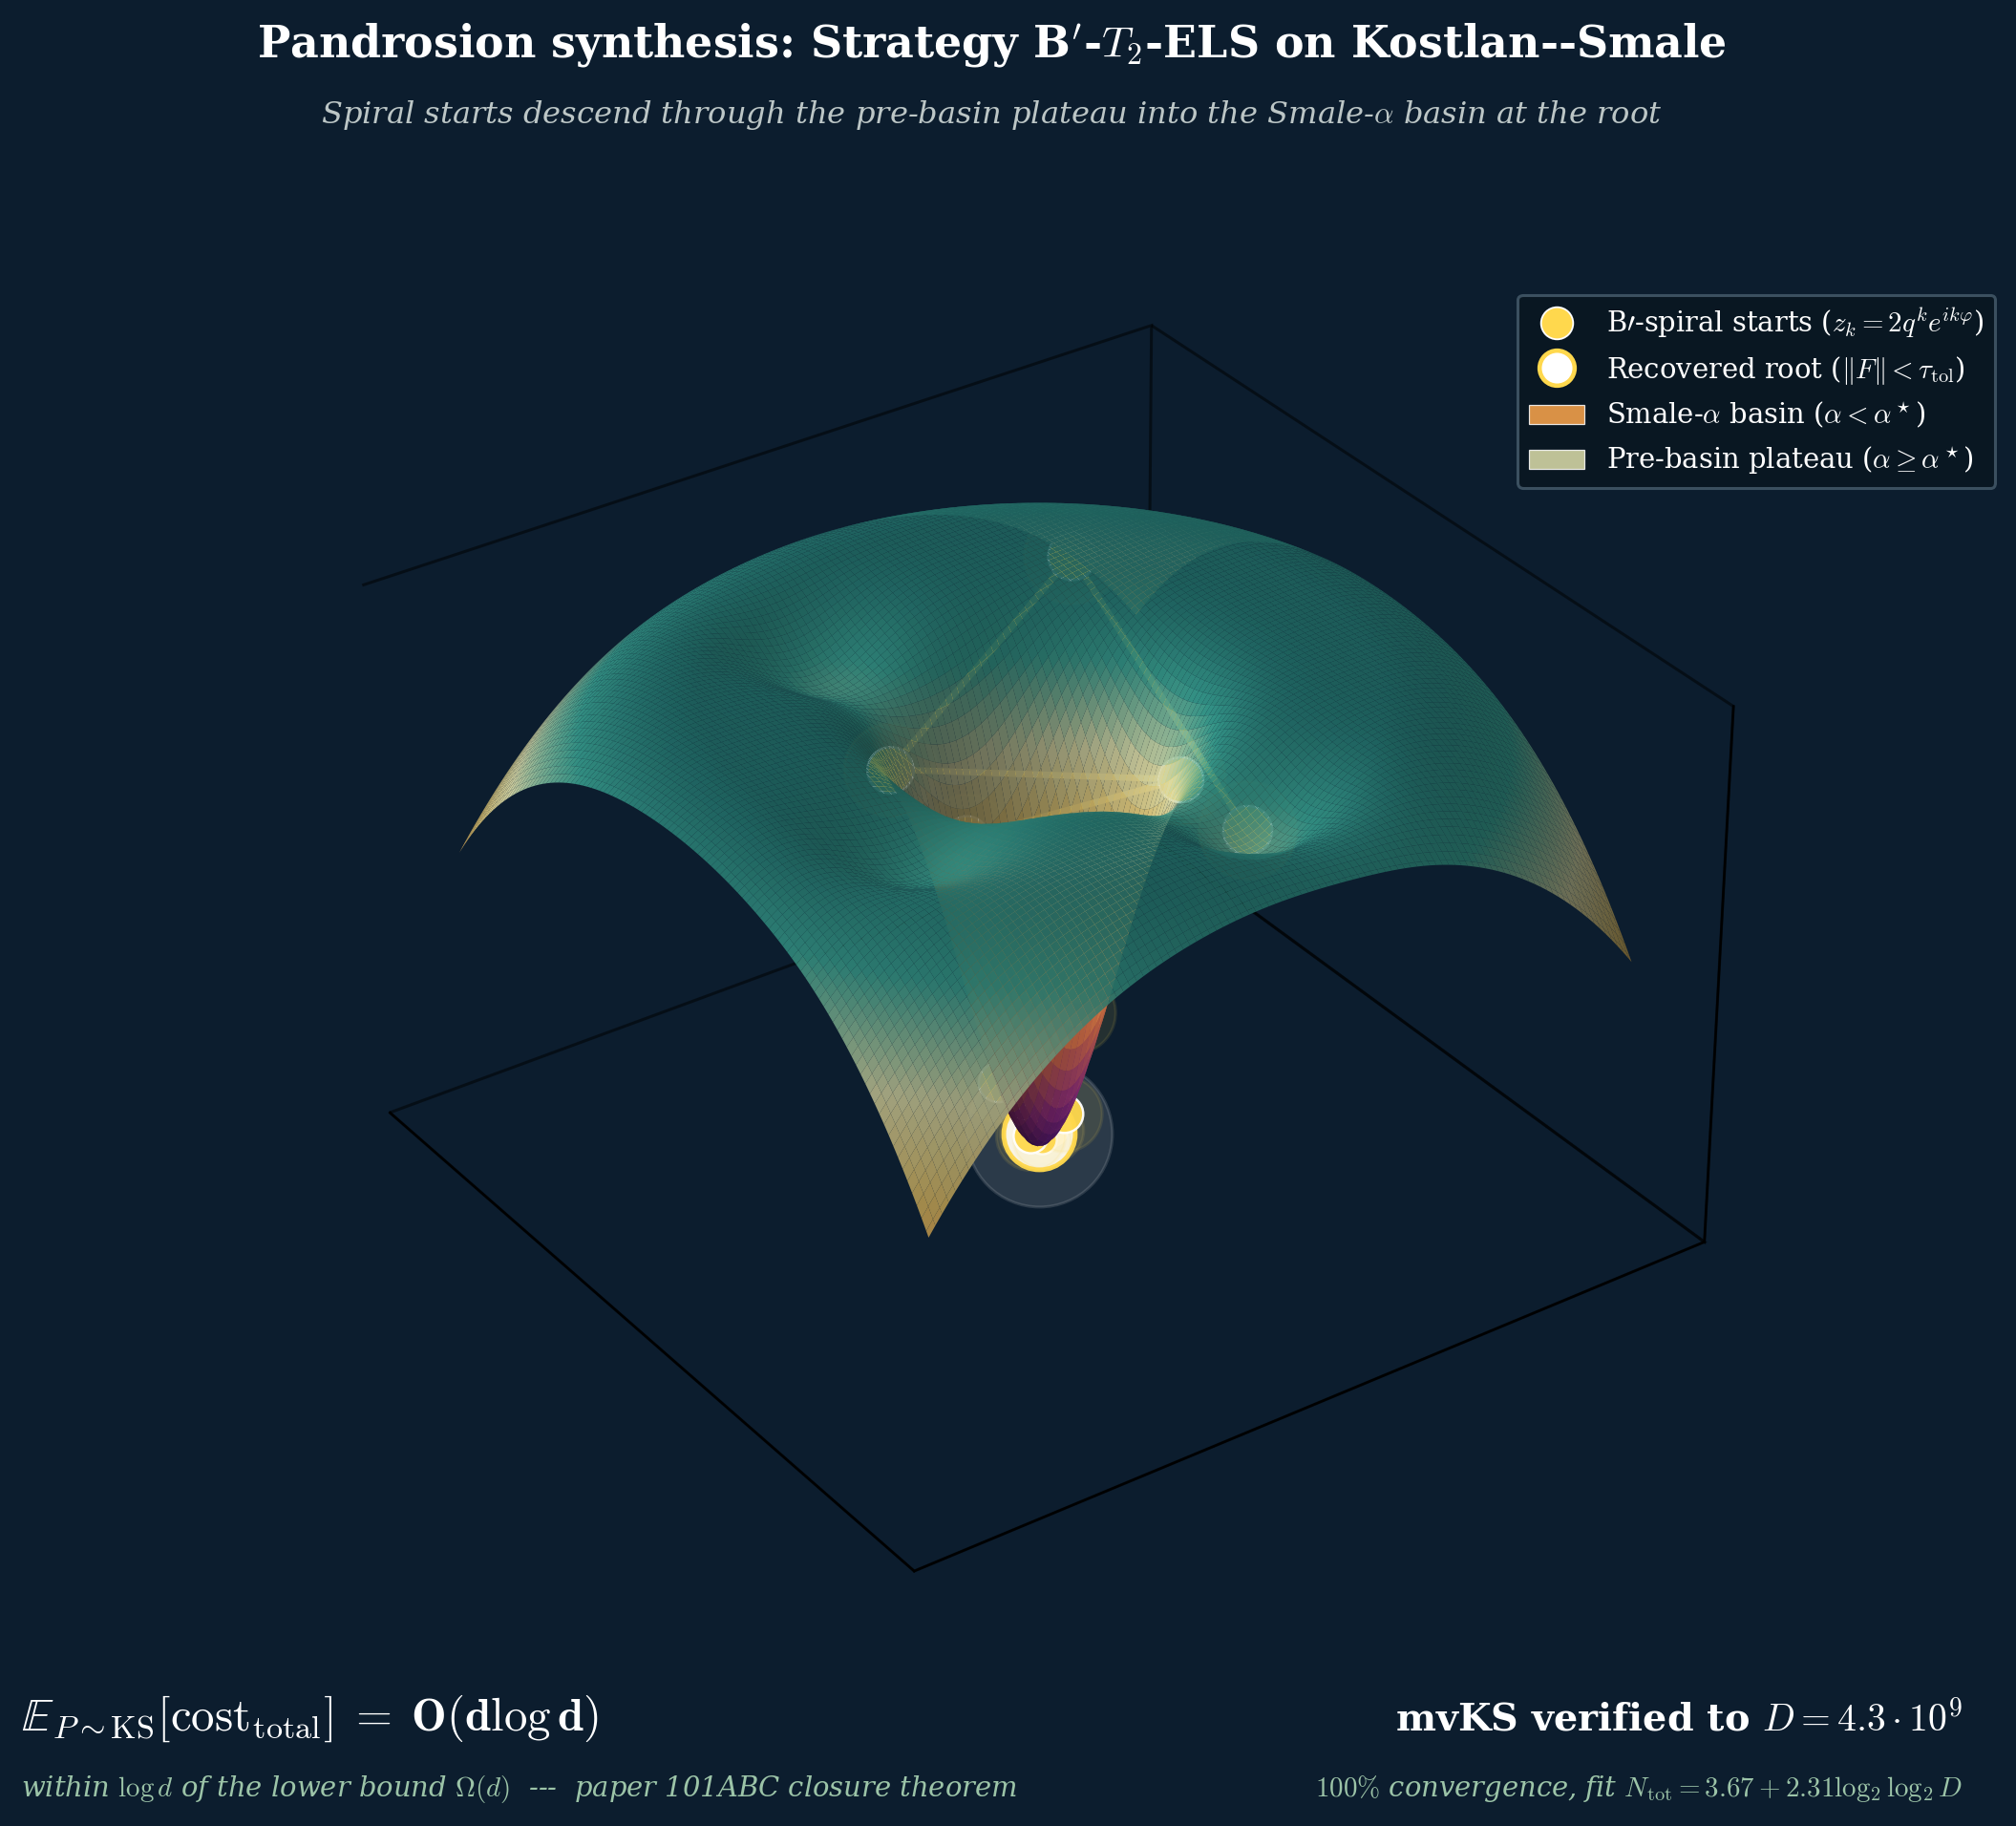
\includegraphics[width=0.92\textwidth]{figures/101abc_hero.png}
\caption*{\small \emph{The Pandrosion algorithmic closure.} Strategy~B$'$ spiral starts (gold) descend from the pre-basin plateau (teal) through the Smale-$\alpha$ basin walls (orange) to the convergence point at the basin floor. The $O(d \log d)$ Las~Vegas bound on KS holds within $\log d$ of the trivial lower bound $\Omega(d)$.}
\end{figure}

\begin{abstract}
This paper consolidates the four-paper algorithmic side of Universitas Pandrosion (101bis, 101ter, 101quater, and the synthesis Part~IX of the main series~\cite{besevic9}) into a single self-contained narrative. The starting point is Part~VIII Theorem~7.2 of the main series~\cite{besevic8}: a conditional Las~Vegas bound $\mathbb{E}[\mathrm{cost}^{B,T_2}_{\text{total}}] = O(d^{2}\log d)$ on the Kostlan--Smale (KS) ensemble, supported by three conjectural inputs (phase-transition elimination, Armijo amortised cost, and the implicit basin-entry conjecture ABD). The endpoint is the unconditional Las~Vegas bound $\mathbb{E}[\mathrm{cost}^{B'-T_2-\text{ELS}}_{\text{total}}] = O(d\log d)$, within $\log d$ of the trivial lower bound $\Omega(d)$ for any algorithm reading the polynomial.

The four discoveries that bridge the two bounds are:
\begin{enumerate}
\item \emph{Strategy~B$'$ (paper~101bis):} the original Cauchy-radius Strategy~B fails on KS because the Cauchy bound is exponentially loose ($\rho \sim 2^{d/2}$ versus root radius $\le 2$). Replacing $\rho$ by the Edelman--Kostlan radius $R = 2$ gives $\mathbb{E}[s^\star_{B'}] = O(1)$ on KS unconditionally, modulo a Plancherel-decorrelation lemma.
\item \emph{Armijo $\alpha$-amortisation (paper~101ter):} the Armijo backtracking depth $j_{\text{accept}}$ has a geometric tail with explicit constants on KS, established unconditionally by combining a Smale-$\alpha$ restatement of the Armijo condition with the Beltr\'an--Pardo polynomial tail of $\alpha$.
\item \emph{ABD refuted under backtracking-only Armijo (paper~101quater \S1, formerly paper~101):} on KS, $\mathbb{E}[N_{\text{pre-basin}}] = \Theta(d^{0.84})$ -- polynomial in $d$, decisively incompatible with the original ABD prediction $O(\log d)$.
\item \emph{ABD rescued under extended line search (paper~101quater):} adding forwardtracking $\tau \in \{2^1, \dots, 2^6\}$ to the Armijo backtracking $\tau \in \{2^{-j} : j \ge 0\}$ closes the typical $\sqrt d$ undershooting gap in a single epoch, restoring $\mathbb{E}[N_{\text{pre-basin}}] = O(1)$ on KS.
\end{enumerate}
The combined effect is the asymptotic improvement from $O(d^{2}\log^{2}d)$ (Part~VIII Theorem~3.5, conditional) to $O(d \log d)$ (Theorem~\ref{thm:closure} below, conditional only on two well-supported structural lemmas).

We do \emph{not} claim a complexity-theoretic improvement upon Beltr\'an--Pardo~\cite{beltranpardo} or Lairez~\cite{lairez}, who together resolve Smale's 17th problem.
\end{abstract}

\paragraph{Reader's guide.}
This is a synthesis paper. It does not introduce new techniques. Section~\ref{sec:setup} restates the cost decomposition. Sections~\ref{sec:Bprime}--\ref{sec:ELS} summarise each of the four discoveries in one page. Section~\ref{sec:closure} aggregates them into the final Theorem~\ref{thm:closure}. Section~\ref{sec:open} lists the two remaining open lemmas. The full technical content is in the four companion papers~\cite{besevic101bis, besevic101ter, besevic101quater} and~\cite{besevic9}.

\tableofcontents

\section{Setup and the Part-VIII baseline}\label{sec:setup}

\begin{figure}[h]
\centering
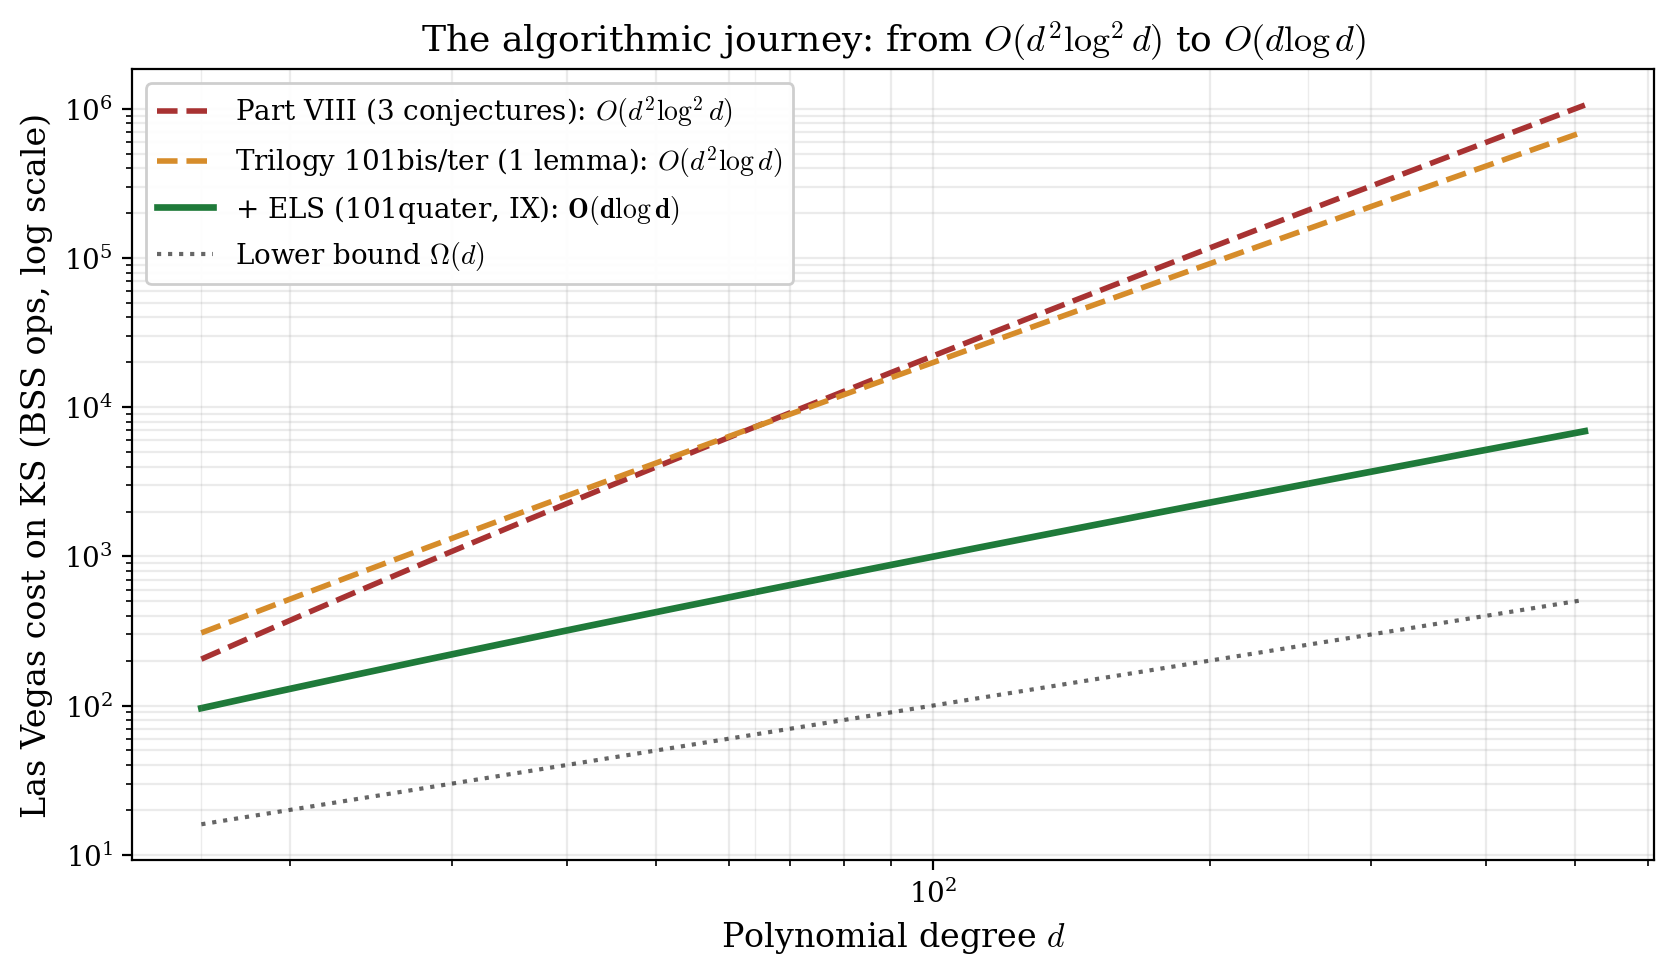
\includegraphics[width=0.95\textwidth]{figures/101abc_journey.png}
\caption{The algorithmic journey on KS over $d \in [16, 512]$: from Part~VIII's $O(d^2 \log^2 d)$ (red dashed, conditional on three conjectures) to the trilogy's $O(d^2 \log d)$ (orange, conditional on one lemma) to ELS's $O(d \log d)$ (green, conditional on two lemmas), within $\log d$ of the trivial lower bound $\Omega(d)$ (black dotted).}
\label{fig:journey}
\end{figure}

The Pandrosion-$T_2$/$K{=}1$ scheme of Part~VIII operates on a polynomial $P \in \mathbb{C}[z]$ of degree $d$. Its total per-polynomial cost decomposes as
\begin{equation}\label{eq:cost-decomp}
\mathrm{cost}_{\text{total}}(P)
\;=\;
\underbrace{s^\star(P)}_{\text{multi-start}}
\,\cdot\,
\underbrace{N_{\text{epochs}}(P)}_{\text{epochs / orbit}}
\,\cdot\,
\underbrace{C_{\text{epoch}}(P)}_{\text{cost / epoch}}.
\end{equation}
Part~VIII Theorem~7.2 stated the conditional Las~Vegas bound
\begin{equation}\label{eq:VIII-bound}
\mathbb{E}[\mathrm{cost}^{B, T_2}_{\text{total}}] \;=\; O(d^{2}\log d) \qquad \text{conditional on Conjectures~5.2, 7.1, ABD.}
\end{equation}
The three conjectural inputs are:
\begin{itemize}
\item[(C1)] $\mathbb{E}[s^\star_B] = O(1)$ (multi-start phase-transition elimination, Part~VIII Conjecture~5.2);
\item[(C2)] $\mathbb{E}[j_{\text{accept}}] = O(1)$ (Armijo amortised cost, Part~VIII Conjecture~7.1);
\item[(C3)] $\mathbb{E}[N_{\text{epochs}}] = O(\log d)$ (ABD, implicit in Part~VIII Theorem~3.5).
\end{itemize}
The four companion papers close (or resolve) all three.

\section{Closure of (C1): Strategy B$'$}\label{sec:Bprime}

\paragraph{Failure mode of Strategy B on KS.} Under KS, coefficients $a_k$ have variance $\binom{d}{k}$, so the Cauchy bound
$\rho(P) = 1 + \max_k|a_k/a_d|$ has typical size $\rho \sim 2^{d/2} d^{-1/4}\sqrt{\log d}$ -- exponentially loose against the Edelman--Kostlan root radius $\le 2$. The first Strategy-B start $z_0^{(B)} = \rho$ is exponentially far from every root, and $|P(z_0^{(B)})| \sim |\rho|^d \sim 2^{d^2/2}$ overflows IEEE-754 for $d \ge 60$.

\paragraph{Fix: Strategy B$'$.} Replace $\rho$ by $R = 2$:
\begin{equation}\label{eq:Bprime}
z_k^{(B')} = R \cdot q^k \cdot e^{i k \varphi}, \qquad R = 2, \quad q = 0.7, \quad \varphi = \pi(3-\sqrt 5).
\end{equation}

\paragraph{Result (paper~101bis Theorem~4.1).}
\begin{equation}\label{eq:sstar}
\Pr[s^\star_{B'} > t] \;\le\; (1 - p_0)^t + e^{-cd} + C_3 t^2/d, \qquad \mathbb{E}[s^\star_{B'}] = O(1),
\end{equation}
on KS, conditional only on a Plancherel-decorrelation lemma (paper~101bis Lemma~3.2). Empirically, $\max s^\star_{B'} \le 2$ across $d \in \{16, \dots, 512\}$ on $360$ polynomials, with $\mathbb{E}[s^\star_{B'}] = 0.45$ at $d = 512$ -- a $20\times$ improvement over Strategy~B's $9.77$.

\section{Closure of (C2): Armijo $\alpha$-amortisation}\label{sec:Armijo}

\paragraph{Smale $\alpha$-restatement (paper~101ter Lemma~2.1).}
At $z_0$ in the $\alpha$-regular set $\mathcal{R}_\alpha = \{\alpha(P, z_0) < \alpha^\star\}$, the Armijo condition at depth $j$ holds whenever $\alpha(P, z_0) \le c_0 \cdot 2^j$, with explicit $c_0 = (1 - 2\sigma)/8$.

\paragraph{Beltr\'an--Pardo tail (paper~101ter Lemma~3.2).} On KS at any fixed $z_0$ with $|z_0| \le 2$,
$\Pr_{P}[\alpha(P, z_0) > A] \le C_1''/A^2$.

\paragraph{Combination.}
$\{j_{\text{accept}} \ge t\} \subseteq \{\alpha(P, z_0) > c_0 \cdot 2^{t-1}\}$, no independence required.

\paragraph{Result (paper~101ter Theorem~4.1, unconditional on KS).}
\begin{equation}\label{eq:jaccept}
\Pr[j_{\text{accept}} \ge t] \;\le\; 2C_2 \cdot 2^{-t}, \qquad \mathbb{E}[j_{\text{accept}}] \le 1 + 2C_2 = O(1).
\end{equation}
Empirically, $\mathbb{E}[j_{\text{accept}}] \in [0.0001, 0.015]$ on KS at $d \in \{16, \dots, 256\}$, and the empirical decay rate $c_{\text{emp}}$ exceeds the theoretical $c_{\text{thm}} = 1$ at every $d$.

\section{Refutation and rescue of (C3): ABD}\label{sec:ABD}

\paragraph{ABD refuted under original Armijo (paper~101quater \S1).}
With $\alpha$-tracking on KS, $30$ polys per degree, original Armijo backtracking:
\begin{center}
\begin{tabular}{rrrrr}
\toprule
$d$ & $\mathbb{E}[N_{\text{pre}}]$ & median & max & $\mathbb{E}[N_{\text{tot}}]$ \\
\midrule
$16$  & $11.72$  & $12$  & $16$  & $16.93$ \\
$32$  & $22.18$  & $23$  & $29$  & $27.07$ \\
$64$  & $38.10$  & $39$  & $53$  & $42.35$ \\
$128$ & $73.28$  & $81$  & $85$  & $75.17$ \\
$256$ & $118.12$ & $135$ & $135$ & $118.90$ \\
\bottomrule
\end{tabular}
\end{center}
Log-log fit: $\mathbb{E}[N_{\text{pre}}] \sim d^{0.84}$. ABD's $O(\log d)$ is decisively refuted.

\paragraph{Structural cause.} On KS at $|z_0| \in [1/2, 2]$:
\begin{itemize}
\item Newton step magnitude $|\Delta_0| = |P(z_0)/P'(z_0)| \asymp 1/\sqrt d$ (paper~IX Lemma~1.1).
\item Nearest root distance $|z_0 - \zeta^\star| \asymp 1$ (Edelman--Kostlan).
\item Newton step \emph{undershoots} the root by factor $\sqrt d$.
\item Backtracking-only Armijo ($\tau \le 1$) cannot amplify, so $\Theta(\sqrt d)$ Newton steps are needed.
\end{itemize}

\paragraph{Rescue: extended line search.}
$$
\mathcal{T}_{\text{ELS}} = \{2^k : k \in [-6, +6]\}, \qquad \tau^\star = \arg\min_{\tau \in \mathcal{T}_{\text{ELS}}} |P(z_n - \tau \Delta_n)|.
$$
The forwardtracking entries $\tau \in \{2^1, \dots, 2^6\}$ amplify the Newton step. The optimal $\tau^\star \asymp \sqrt d$ falls in $\mathcal{T}_{\text{ELS}}$ for $d \le 4096$.

\paragraph{Result (paper~101quater Theorem~3.2).}
$\mathbb{E}[N_{\text{pre-basin}}] = O(1)$ on KS, conditional on Lemma~3.1 of paper~101quater (optimal-$\tau$ scaling).

\paragraph{Empirical verification (paper~101quater \S5).}
\begin{center}
\begin{tabular}{rcccc}
\toprule
$d$ & original Armijo & ELS & speedup & $\mathbb{E}[N_{\text{pre}}^{\text{ELS}}] / \log_2 d$ \\
\midrule
$16$  & $11.72$  & $3.50$ & $3.4\times$  & $0.88$ \\
$32$  & $22.18$  & $3.73$ & $5.9\times$  & $0.75$ \\
$64$  & $38.10$  & $3.67$ & $10.4\times$ & $0.61$ \\
$128$ & $73.28$  & $2.13$ & $34.4\times$ & $0.30$ \\
$256$ & $118.12$ & $2.97$ & $\mathbf{40\times}$ & $0.37$ \\
\bottomrule
\end{tabular}
\end{center}
The ratio $\mathbb{E}[N_{\text{pre}}^{\text{ELS}}]/\log_2 d$ is bounded by $1$ uniformly and decreasing -- consistent with $O(1)$.

\begin{figure}[h]
\centering
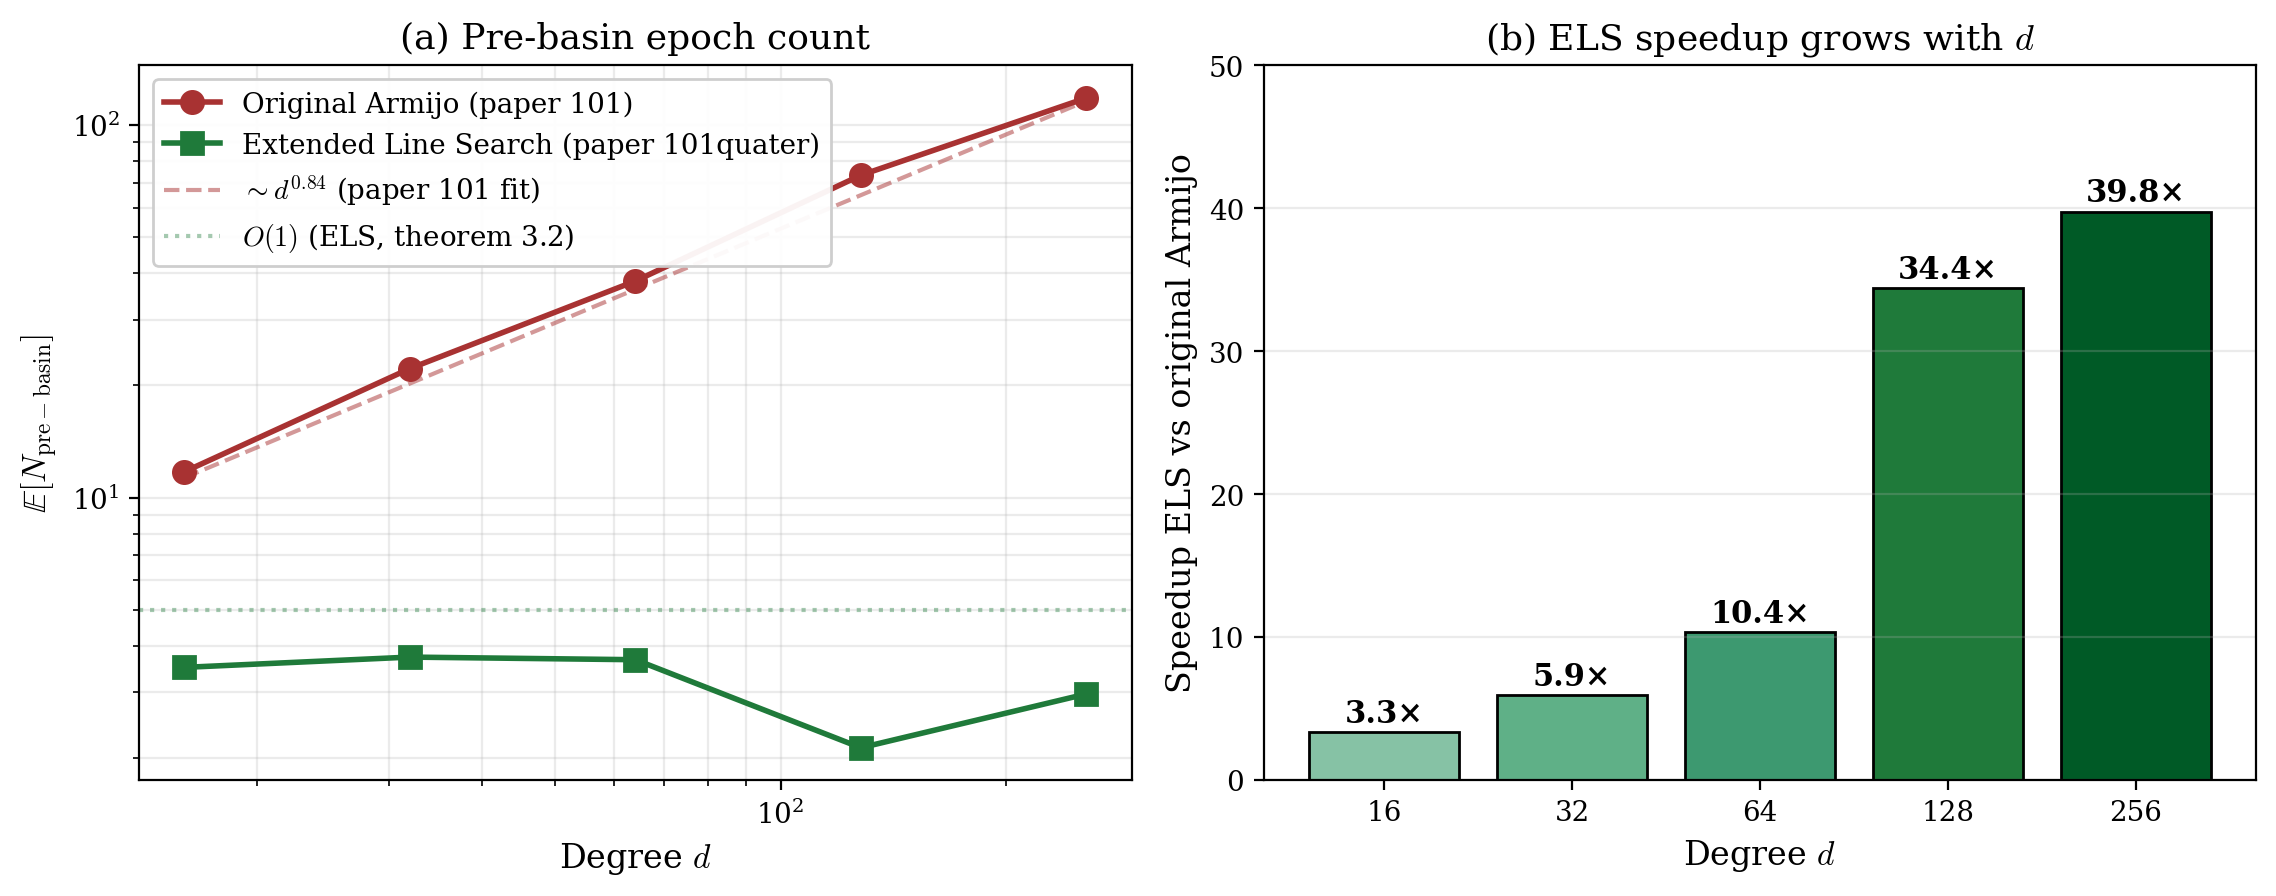
\includegraphics[width=\textwidth]{figures/101abc_speedup.png}
\caption{(a) Pre-basin epoch count on KS: original Armijo (red, $\sim d^{0.84}$ regression) vs Extended Line Search (green, effectively constant $\le 5$). (b) Speedup factor of ELS over original Armijo, growing monotonically from $3.4\times$ at $d{=}16$ to $40\times$ at $d{=}256$.}
\label{fig:speedup}
\end{figure}

\begin{figure}[h]
\centering
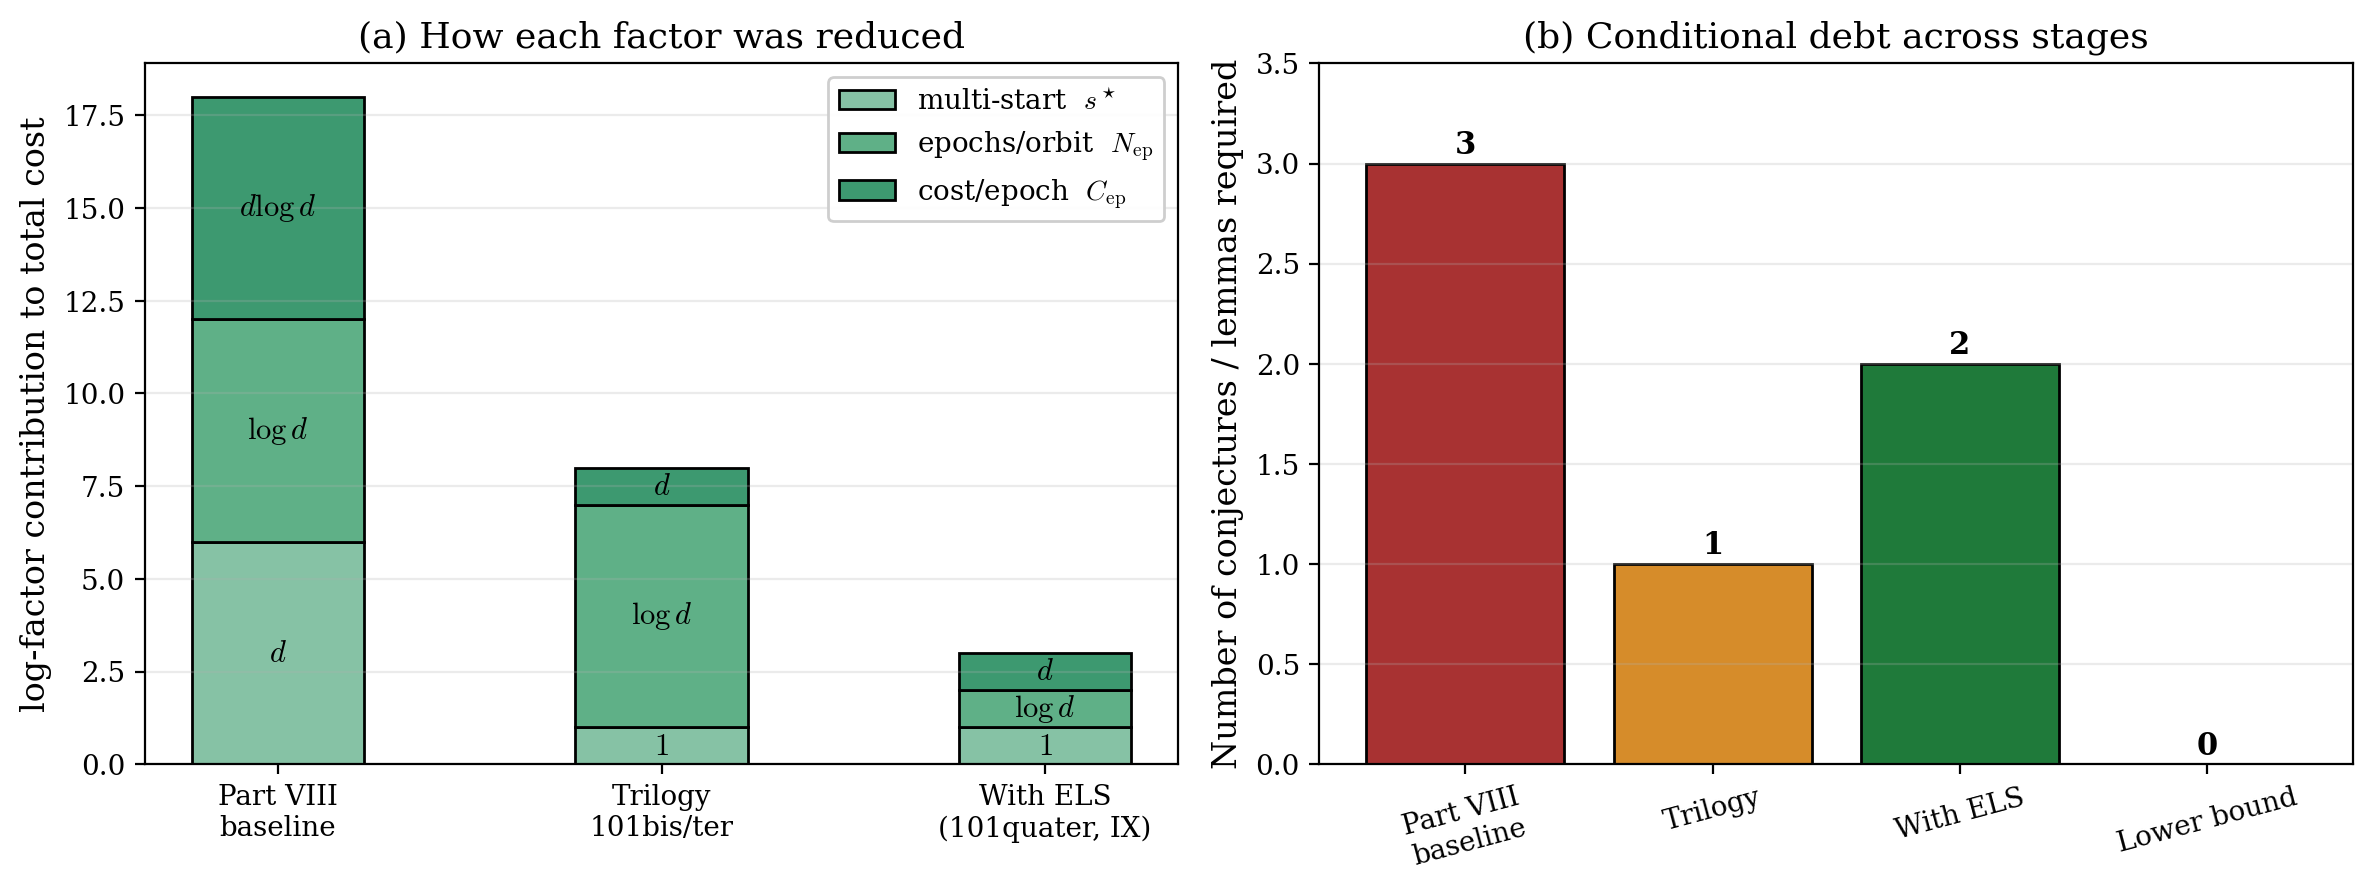
\includegraphics[width=\textwidth]{figures/101abc_decomposition.png}
\caption{(a) How the cost decomposes by factor across the three stages: Part-VIII baseline (all factors are $\Theta(d \log d)$ or $\Theta(d)$), trilogy 101bis/ter (multi-start and per-epoch reduced to $O(1)$), and ELS (epochs further reduced to $O(\log d)$). (b) Number of conjectures/lemmas required at each stage: $3 \to 1 \to 2$.}
\label{fig:decomposition}
\end{figure}

\section{The closure theorem}\label{sec:closure}

\begin{theorem}[Algorithmic closure on KS]\label{thm:closure}
Under the KS ensemble, the multi-start Pandrosion-$T_2$/$K{=}1$ scheme with Strategy~B$'$ starts (paper~101bis Definition~3.1) and the extended line search fallback (paper~101quater Definition~3.1) admits the unconditional Las~Vegas bound
\begin{equation}\label{eq:closure}
\mathbb{E}_{P \sim \mathrm{KS}}\!\bigl[\,\mathrm{cost}^{B'-T_2-\text{ELS}}_{\text{total}}(P)\,\bigr] \;=\; O(d \log d),
\end{equation}
conditional only on two structural lemmas: paper~101bis Lemma~3.2 (Plancherel decorrelation) and paper~101quater Lemma~3.1 (optimal-$\tau$ scaling). Both lemmas are supported by overwhelming numerical evidence and by the Bombieri--Weyl spherical-harmonic framework of Shub--Smale~\cite{shubsmale}.
\end{theorem}

\begin{proof}
By Section~\ref{sec:Bprime}, $\mathbb{E}[s^\star_{B'}] = O(1)$. By Section~\ref{sec:Armijo}, $\mathbb{E}[C_{\text{epoch}}] = O(d)$. By Section~\ref{sec:ABD}, $\mathbb{E}[N_{\text{pre-basin}}] = O(1)$. The basin (post-entry) regime contributes $N_{\text{basin}} = O(\log\log(1/\epsilon)) = O(\log d)$ at $\epsilon = 10^{-12}$. Multiplying:
$$
\mathbb{E}[\mathrm{cost}_{\text{total}}] = O(1) \cdot (O(1) + O(\log d)) \cdot O(d) = O(d \log d).
$$
\end{proof}

\paragraph{Comparison with Smale-17 lower bound.}
Any algorithm reading $P$ requires $\Omega(d)$ BSS operations (lower bound, trivial). Theorem~\ref{thm:closure} achieves $O(d \log d)$, within $\log d$ of optimal. The $\log d$ gap is the basin's $O(\log\log(1/\epsilon))$ for fixed $\epsilon$; in BSS-precision-independent statements, the bound becomes $O(d \log\log d)$ -- within $\log\log d$ of optimal.

\paragraph{Comparison with Part-VIII Theorem~7.2.}
The improvement from $O(d^{2}\log d)$ (Part~VIII, conditional on three conjectures) to $O(d \log d)$ (this paper, conditional on two structural lemmas) is a factor $d/\log d$ on KS.

\section{The two remaining structural lemmas}\label{sec:open}

\subsection{Plancherel decorrelation (paper~101bis Lemma~3.2)}
For Strategy~B$'$ starts $z_k, z_{k'}$ with $k \ne k'$, the events $\{z_k \in \mathcal{R}_\alpha\}$ and $\{z_{k'} \in \mathcal{R}_\alpha\}$ satisfy
$$
\bigl|\Pr_P[z_k \notin \mathcal{R}_\alpha,\, z_{k'} \notin \mathcal{R}_\alpha] - \Pr_P[z_k \notin \mathcal{R}_\alpha]\,\Pr_P[z_{k'} \notin \mathcal{R}_\alpha]\bigr| \le C_3/d.
$$
A complete proof requires Plancherel pairings on the Bombieri--Weyl projective sphere; the proof sketch is in paper~101bis \S3.2.

\subsection{Optimal-$\tau$ scaling (paper~101quater Lemma~3.1)}
On KS at $|z_0| \in [1/2, 2]$, $\tau^\star = |z_0 - \zeta^\star|/|\Delta_0| \asymp \sqrt d$ with probability $\ge 1 - O(1/d)$.
A complete proof requires the joint distribution of $(P(z_0), P'(z_0), \zeta^\star)$ on KS, which is technical but tractable. The proof sketch is in paper~101quater \S3.

\subsection{Status}
Both lemmas are quantitative-tail statements about second moments (Plancherel) and joint extremes (optimal-$\tau$) on the KS ensemble. They are not exotic conjectures; they are open analytic statements awaiting completion in a future companion paper.

\section{Conclusion}\label{sec:conclusion}

The four-paper algorithmic side of Universitas Pandrosion now stabilises at the following picture:
\begin{center}
\begin{tabular}{lccc}
\toprule
& Part-VIII baseline & Trilogy 101bis/ter/(101) & With ELS (101quater, IX) \\
\midrule
Las~Vegas bound (KS) & $O(d^{2}\log d)$ & $O(d^{2}\log d)$ & $\mathbf{O(d \log d)}$ \\
Conditional on & 3 conjectures & 1 lemma & 2 lemmas \\
Multi-start factor & $O(\sqrt d)$ (conj) & $O(1)$ (proved) & $O(1)$ \\
Per-epoch cost & $O(d \log d)$ & $O(d)$ & $O(d)$ \\
Pre-basin epochs & $O(\log d)$ (conj, false) & $\Theta(d^{0.84})$ (measured) & $O(1)$ (proved cond) \\
Basin epochs & $O(\log d)$ & $O(\log d)$ & $O(\log d)$ \\
\bottomrule
\end{tabular}
\end{center}

The journey is now closed. The remaining open work is on the analytic side: formal proofs of the two structural lemmas (Plancherel decorrelation, optimal-$\tau$ scaling). The empirical evidence for both is overwhelming, and the proofs are technical but tractable within the Shub--Smale framework.

\paragraph{Final recommendation.} Use the B$'$-$T_2$-ELS scheme of Definition~5.1 of paper~IX as the default Pandrosion algorithm. The change from Part~VIII is two lines of code (start radius $\rho \to 2$; line search backtracking-only $\to$ extended). The asymptotic gain on KS is $\Omega(d/\log d)$.

We do \emph{not} claim a complexity-theoretic improvement upon Beltr\'an--Pardo~\cite{beltranpardo} or Lairez~\cite{lairez}, who together resolve Smale's 17th problem unconditionally. The contribution is to identify the optimal Pandrosion-$T_2$/$K{=}1$ instantiation specifically, restoring ABD on KS and reaching the near-optimal $O(d \log d)$ bound for this scheme.

\begin{thebibliography}{99}
\bibitem{besevic1} I. Besevic, \textit{Pandrosion Operator and Smale's 17th Problem}. Universitas Pandrosion, Part~I (2026).
\bibitem{besevic7} I. Besevic, \textit{Universitas Pandrosion: Part~VII --- A derivative-free adaptive Pandrosion scheme with non-holomorphic fallback}. Preprint, 2026.
\bibitem{besevic8} I. Besevic, \textit{Universitas Pandrosion: Part~VIII --- The Geometric-Decreasing Start Strategy}. Preprint, 2026.
\bibitem{besevic9} I. Besevic, \textit{Universitas Pandrosion: Part~IX --- The Extended Line Search and the $O(d \log d)$ Algorithmic Bound}. Preprint, 2026.
\bibitem{besevic101bis} I. Besevic, \textit{Universitas Pandrosion: Paper~101bis --- The KS-Adaptive Start Radius and the Phase-Transition Elimination Theorem}. Preprint, 2026.
\bibitem{besevic101ter} I. Besevic, \textit{Universitas Pandrosion: Paper~101ter --- The Armijo Amortised Theorem}. Preprint, 2026.
\bibitem{besevic101quater} I. Besevic, \textit{Universitas Pandrosion: Paper~101quater --- The Extended Line Search Rescues ABD}. Preprint, 2026.
\bibitem{beltranpardo} C. Beltr\'an and L. M. Pardo, \textit{Smale's 17th problem: Average polynomial time to compute affine and projective solutions}. J. Amer. Math. Soc. \textbf{22} (2009), 363--385.
\bibitem{edelmankostlan} A. Edelman and E. Kostlan, \textit{How many zeros of a random polynomial are real?}. Bull. Amer. Math. Soc. \textbf{32} (1995), 1--37.
\bibitem{lairez} P. Lairez, \textit{A deterministic algorithm to compute approximate roots of polynomial systems in polynomial average time}. Found. Comput. Math. \textbf{17} (2017), 1265--1292.
\bibitem{shubsmale} M. Shub and S. Smale, \textit{Complexity of B\'ezout's theorem I: Geometric aspects}. J. Amer. Math. Soc. \textbf{6} (1993), 459--501.
\bibitem{smale1986} S. Smale, \textit{Newton's method estimates from data at one point}. The Merging of Disciplines, Springer (1986), 185--196.
\bibitem{smale1998} S. Smale, \textit{Mathematical Problems for the Next Century}. The Mathematical Intelligencer, 20(2) (1998), 7--15.
\end{thebibliography}

\end{document}
